
\begin{figure*}[t]
     \centering
     \begin{subfigure}[b]{0.48\textwidth}
         \centering
         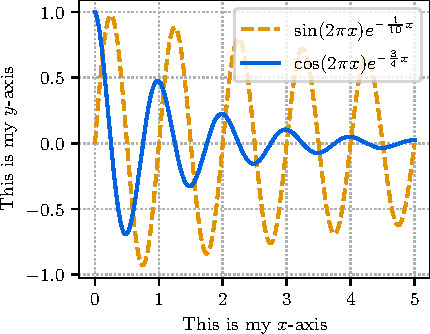
\includegraphics[]{assets/plot_demo.pdf}
         \caption{First plot.}
         \label{fig:plots:a}
     \end{subfigure}
     \hfill
     \begin{subfigure}[b]{0.48\textwidth}
         \centering
         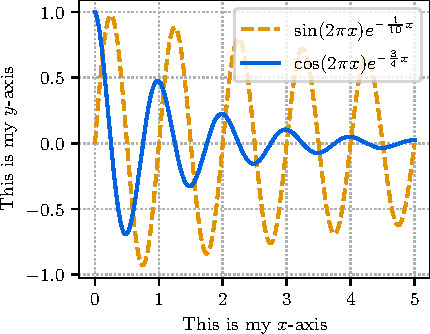
\includegraphics[]{assets/plot_demo.pdf}
         \caption{Second plot.}
         \label{fig:plots:b}
     \end{subfigure}
     \caption{Plots generated with the script \texttt{nice\_plot.py} included in this template.
     % 
     For more information on producing figures, please refer to \href{https://fb.workplace.com/notes/1767028093764250}{this Workplace post}.
     %
     If you would like to use a figure teaser, place it immediately after \texttt{\textbackslash{}maketitle}, forcing its location with the \texttt{[h!]} optional argument.
     %
     Please consider using the \href{https://www.facebook.com/brand/meta/color/}{Meta palette} to color your figures.
     }
     \label{fig:plots}
\end{figure*}